\documentclass{article}

% Language setting
\usepackage[polish]{babel}

% Set page size and margins
% Replace `letterpaper' with `a4paper' for UK/EU standard size
\usepackage[letterpaper,top=2cm,bottom=2cm,left=3cm,right=3cm,marginparwidth=1.75cm]{geometry}

% Useful packages
\usepackage{amsmath}
\usepackage{graphicx}
\usepackage[T1]{fontenc}
\usepackage[colorlinks=true, allcolors=blue]{hyperref}
\usepackage{lipsum}
\usepackage{multicol}
\usepackage{tikz,tcolorbox}
\usepackage{float}

\title{Metoda klasyfikacji cukierków na podstawie ich opakowania}
\author{Aleksander Golus, Bartosz Chadryś, Jakub Miśko, Igor Joński}

\begin{document}
\maketitle

\begin{abstract}
Praca przedstawia metodę klasyfikacji cukierków na podstawie ich opakowania. W tym celu został stworzony układ pomiarowy z taśmy produkcyjnej, kamery oraz zestawu konkretnych cukierków o kolorowych opakowaniach. Następnie została stworzona metoda rozróżniająca i zliczająca opakowania cukierków na podstawie ich koloru.
\end{abstract}

\section{Temat projektu}
\label{Temat projektu}
\definecolor{my-red-light}{RGB}{254, 218, 212}
\definecolor{my-red-dark}{RGB}{220, 97, 85}
\definecolor{my-orange-light}{RGB}{252, 236, 189}
\definecolor{my-orange-dark}{RGB}{247, 167, 9}
\definecolor{my-pink-light}{RGB}{252, 218, 229}
\definecolor{my-pink-dark}{RGB}{247, 132, 168}
\definecolor{my-green}{RGB}{141, 189, 16}


Tematem projektu jest klasyfikacja cukierków na podstawie koloru ich opakowania. W tym celu został stworzony układ pomiarowy z taśmy produkcyjnej, kamery oraz zestawu konkretnych, prostokątnych, cukierków o kolorowych opakowaniach. Następnie została stworzona metoda rozróżniająca opakowania cukierków na podstawie ich koloru oraz zliczająca wystąpienia tych opakowań na podstawie ich koloru.

\section{Wstęp}
\label{Wstęp}
W projekcie opracowano metodę, która pozwala na rozpoznawanie kolorowych opakowań cukierków oraz zliczanie ich wystąpień na linii produkcyjnej. Podstawą metody jest analiza obrazu, w której kluczową rolę odgrywa detekcja kolorów i określenie obszaru zajmowanego przez obiekt. Następnie, korzystając z zaprogramowanych algorytmów, system klasyfikuje cukierki na podstawie barwy opakowań i agreguje dane dotyczące ich ilości.

Metoda ta znajduje zastosowanie w przemyśle spożywczym, zwłaszcza w automatyzacji procesów pakowania oraz kontroli jakości. Umożliwia ona nie tylko szybką selekcję produktów, ale także może przyczynić się do usprawnienia procesów magazynowania i dystrybucji.

Jednym z podobnych rozwiązań z tej branży (spożywczej) jest rozpoznawanie rodzajów bułek oraz ich kształtów tak jak zostało to przedstawione w \cite{virtuslab}, w przypadku tematu, jakim są cukierki, można znaleźć zastosowania w pomocy rozróżniania rodzaju cukierka w bombonierce \cite{chocolates}. Innym przypadkiem użycia detekcji obiektów na podstawie ich opakowania może być również przedstawiona tutaj \cite{vending} innowacyjna metoda rozpoznawania produktów w automatach sprzedających.

\section{Materiały i metody}
\label{Materiały i metody}
\subsection{Materiały badawcze}
\label{Materiały pomiarowe}
Materiałami pomiarowymi są konkretne rodzaje cukierków o kolorowych opakowaniach, to znaczy - cukierki marki Mamba oraz Turbo. Zostały one wybrane ze względu na to, że posiadają bardzo podobny rozmiar, co zdecydowanie ułatwiło implementację metody.

Wykorzystywane cukierki dzielimy na 4 typy kolorów, z czego różowy, czerwony oraz pomarańczowy to cukierki marki Mamba, natomiast zielony - marki Turbo. Cukierki marki Mamba posiadają dwie barwy danego koloru - barwę jaśniejszą oraz ciemniejszą.

\begin{figure}[H]
    \centering
    \begin{tcolorbox}[colback=white]

    \begin{multicols}{4}
    Różowy cukierek
    \begin{tcolorbox}[colback=my-pink-dark, width=\linewidth, colframe=my-pink-dark]
    \end{tcolorbox}
    Czerwony cukierek
    \begin{tcolorbox}[colback=my-red-dark, width=\linewidth, colframe=my-red-dark]
    \end{tcolorbox}
    Pomarańczowy cuk.
    \begin{tcolorbox}[colback=my-orange-dark, width=\linewidth, colframe=my-orange-dark]
    \end{tcolorbox}
    Zielony cukierek
    \begin{tcolorbox}[colback=my-green, width=\linewidth, colframe=my-green]
    \end{tcolorbox}
    \end{multicols}

    \begin{multicols}{4}
    \begin{tcolorbox}[colback=my-pink-light, width=\linewidth, colframe=my-pink-light]
    \end{tcolorbox}
    \begin{tcolorbox}[colback=my-red-light, width=\linewidth, colframe=my-red-light]
    \end{tcolorbox}
    \begin{tcolorbox}[colback=my-orange-light, width=\linewidth, colframe=my-orange-light]
    \end{tcolorbox}
    \end{multicols}

    \end{tcolorbox}
    \caption{Wizualizacja barw dla każdego koloru badanego cukierka}
\end{figure}






\subsection{Przedziały kolorów rozpoznawalnych cukierków}

Kolory cukierków w odpowiednim oświetleniu (omówionym w sekcji \ref{Układ pomiarowy}) powinny zawierać się w następujących zakresach:

\begin{table}[H]
    \label{tab:my_label}
    \centering
    \begin{tabular}{ |c|c|c|c| }
     \hline
     Kolor & Dolna granica & Górna granica \\
     \hline
     Różowy & \#32282f & \#ff0000 \\
     \hline
     Czerwony & \#645050 & \#ff7a37 \\
     \hline
     Pomarańczowy & \#644b3d & \#ffd500 \\
     \hline
     Zielony & \#323222 & \#00ff00 \\
     \hline
    \end{tabular}
    \caption{Przedziały barw, w których musi znaleźć się kolor opakowania cukierka by został zidentyfikowany.}
\end{table}

Wtedy cukierki są rozpoznawane przez program jako cukierki, a nie jako tło.

\subsection{Układ pomiarowy}
\label{Układ pomiarowy}

Układ pomiarowy składa się z ciemnozielonej taśmy produkcyjnej napędzanej silnikiem elektrycznym o stałej prędkości, kamery o rozdzielczości 1080p oraz lampy LED naświetlającej taśmę z góry.
Taśma produkcyjna charakteryzuje się szerokością 10cm oraz stałą prędkością 3cm/s. Oświetlona została lampą ledową o mocy 10W i temperaturze 3500K, co skutkuje klarownym oświetleniem bez zaburzenia kolorów cukierków.
Kamera została ustawiona 20cm nad taśmą, rejestrując przy tym całą szerokość taśmy.
Układ pomiarowy został przedstawiony na rysunku \ref{fig:uklad_pomiarowy}.

\subsection{Metoda pomiarowa}
\label{Metoda pomiarowa}
\subsubsection{Idea}
\label{Idea}

Ideą metody pomiarowej jest zliczanie cukierków występujących na taśmie produkcyjnej bazując na kolorze opakowania cukierka. Przypadki użycia metody pomiarowej to między innymi:

\begin{itemize}
    \item Weryfikacja serii cukierków - czy ilość wyprodukowanych cukierków jest zgodna z ilością cukierków bezpośrednio przed
    \item Weryfikacja serii cukierków - czy ilość cukierków na taśmie jest wystarczająco różnorodna
\end{itemize}

\subsubsection{Sposób pomiaru}
\label{Sposób pomiaru}

Metoda pomiarowa wymaga odpowiedniego umieszczenia kamery nad taśmą produkcyjną (patrz sekcja \ref{Układ pomiarowy}) wraz z odpowiednim oświetleniem. Oprócz tego, metoda wymaga użycia odpowniednich cukierków (patrz sekcja \ref{Materiały pomiarowe}). Cukierek, oprócz odpowiedniego koloru musi również spełniać wymagania dotyczące jego wymiarów, to jest - jego pole powierzchni musi być większe niż 30000 pikseli, w przeciwnym wypadku cukierek zostanie uznany za tło.

\subsection{Wykorzystane narzędzia}
\label{Wykorzystane narzędzia}

\subsubsection{OpenCV-python (cv2)}
\label{OpenCV-python (cv2)}

Wykorzystane metody:
\begin{enumerate}
\item VideoCapture() \cite{opencv1}

Metoda pozwala na otworzenie pliku wideo, obrazu lub uchwycenia obrazu wideo poprzez przesyłanie z innego urządzenia

Użyte parametry:
\begin{itemize}
\item const String \&filename - nazwa pliku
\end{itemize}

\item isOpened() \cite{opencv2}

Metoda używana w celu sprawdzenia czy dany plik wideo lub obraz jest otworzony. Zwraca true, jeśli plik został poprawnie otworzony.

\item read() \cite{opencv3}

Metoda pobiera, dekoduje, a następnie zwraca następną klatkę wideo w postaci dwóch zmiennych retval oraz image.

Opis zwróconych zmiennych:
\begin{itemize}
\item retval - zmienna typu boolean opisująca czy poprawnie udało się odczytać klatkę wideo
\item image - odczytany obraz w postaci tablicy numpy
\end{itemize}

\item cvtColor() \cite{opencv4}

Metoda służy do zmiany przestrzeni barw dla danego obrazu np. z HSV na RGB

Użyte parametry:
\begin{itemize}

\item src - obraz w postaci tablicy numpy, dla którego zmieniamy przestrzeń barw
\item code - kod z biblioteki cv2 opisujący zmianę przestrzeni barw np. COLOR\_BGR2HSV, czyli zmiana z barw BGR na HSV

\end{itemize}

\item imshow() \cite{opencv5}

Metoda pozwala na wyświetlenie obrazu w oddzielnym oknie programu. Okno automatycznie dostosowywuje się do rozmiaru obrazu.

Użyte parametry:
\begin{itemize}
\item window\_name - parametr typu string opisujący nazwę okna
\item image - obraz w postaci tablicy numpy, który zostanie wyświetlony
\end{itemize}

\item waitKey() \cite{opencv6}

Metoda pozwala użytkownikowi na wyświetlenie okna przez dany czas, lub dopóki nie wciśnie danego przycisku. Przyjmuje ona czas w milisekundach, jeśli zostanie przekazane 0, to czeka dopóki dowolny przycisk zostanie wciśnięty

Użyte parametry:
\begin{itemize}
\item delay - parametr opisujący czas w milisekundach
\end{itemize}

\item putText() \cite{opencv7}

Funkcja używana w celu wyświetlenia tekstu na danym obrazie.

Użyte parametry:

\begin{itemize}
\item image - obraz w postaci tablicy numpy na którym zostanie wyświetlony tekst
\item text - dany text typu string który zostanie wyświetlony na obrazie
\item org - parametr typu tuple przechowujący koordynaty w postaci (x, y)
\item font - nazwa fontu z biblioteki cv2 np. FONT\_HERSHEY\_SIMPLEX
\item fontScale - parametr opisujący skalę fontu
\item color - kolor tekstu typu string np. „Red”
\item thickness - grubość tekstu
\end{itemize}

\item findContours() \cite{opencv8}

Metoda pomaga w wydobyciu konturu z obrazu. Najlepiej działa na obrazach binarnych, więc najlepiej zacząć od technik progowania.

Użyte parametry:

\begin{itemize}
\item image - obraz w postaci tablicy numpy dla którego szukamy konturów
\item mode - tryby z biblioteki cv2. Użyliśmy RETR\_EXTERNAL  do wydobycia tylko zewnętrznych konturów oraz CHAIN\_APPROX\_SIMPLE do usuwania zbędnych punktów i kompresowania konturów.
\end{itemize}

\item contourArea() \cite{opencv9}

Funkcja zwracająca pole dla danego konturu przekazanego w parametrze.

Użyte parametry:

\begin{itemize}
\item contour - dany kontur dla którego chcemy uzyskać pole
\end{itemize}

\item boundingRect \cite{opencv10}

Funkcja oblicza i zwraca punkty x,y oraz szerokość i wysokość dla danego obrazu

Użyte parametry:

\begin{itemize}
\item array - obraz w postaci tablicy numpy
\end{itemize}

\item inRange() \cite{opencv11}

Metoda zwracająca przekształconą maskę obrazu dla danego przedziału kolorów na przekazanym obrazie.

Użyte parametry:

\begin{itemize}
\item src - obraz w postaci tablicy numpy
\item lowerb - dolny przedział kolorów od którego chcemy uzyskać maskę
\item upperb - górny przedział kolorów do którego chcemy uzyskać maskę
\end{itemize}

\item rectangle() \cite{opencv12}

Funkcja wyświetlająca prostokąt na przekazanym obrazie.

Użyte parametry:

\begin{itemize}
\item image - obraz w postaci tablicy numpy na którym ma zostać namalowany prostokąt
\item start\_point - punkt w postaci tupli (x, y) gdzie ma się zacząć prostokąt
\item end\_point - punkt w postaci tupli (x, y) gdzie ma się zakończyć prostokąt
\item color - kolor typu string np. „Blue”
\item thickness - grubość prostokąta typu float
\end{itemize}

\item release() \cite{opencv13}

Metoda zamyka plik wideo lub przerywa nagrywanie z danego urządzenia.

\item destroyAllWindows() \cite{opencv14}

Funkcja zamyka wszystkie otwarte okna

\item threshold() \cite{opencv15}

Metoda służy do progowania przekazanego obrazu w parametrze

Użyte parametry:

\begin{itemize}
\item source - obraz w postaci tablicy numpy (musi być w szarości) na którym wykonane zostanie progowanie
\item thresh - wartość progu poniżej i powyżej, przy której wartości pikseli zostaną odpowiednio zmienione
\item maxval - maksymalna wartość, która może zostać przypisana do piksela
\item type - metoda którą zostanie wykonane progowanie np. THRESH\_BINARY
\end{itemize}

\item line() \cite{opencv16}

Funkcja służy do narysowania linii na przekazanym obrazie

Użyte parametry:

\begin{itemize}
\item img - przekazany obraz jako tablica numpy na którym ma zostać wyświetlona linia
\item pt1 - początkowy punkt z którego ma być narysowana linia w postaci tupli (x, y)
\item pt2 - końcowy punkt, gdzie linia powinna się zakończyć w postaci tupli (x, y)
\item color - kolor w postaci string np. „Green”
\item thickness - grubość linii typu float
\end{itemize}

\end{enumerate}

\section{Wyniki i dyskusja}
\label{Wyniki i dyskusja}
Efektywność działania metody została przetestowana na dwóch wcześniej przygotowanych nagraniach taśmy produkcyjnej ze znajdującymi się na niej cukierkami.
\subsection{Nagranie 1}
Analizując rezultaty otrzymaliśmy następujące wyniki:

\begin{center}
\begin{tabular}{|p{0.15\linewidth}|p{0.25\linewidth}|p{0.25\linewidth}|p{0.25\linewidth}|}
 \hline
 Kolor opakowania & Rzeczywista ilość cukierków & Ilość cukierków rozpoznana przez metodę & Procent rozpoznanych cukierków \\
 \hline
 Czerwony & 4 & 4 & 100\% \\
 \hline
 Różowy & 6 & 6 & 100\% \\
 \hline
 Pomarańczowy & 8 & 8 & 100\% \\
 \hline
 Zielony & 7 & 7 & 100\% \\
 \hline
\end{tabular}
\end{center}

\begin{center}
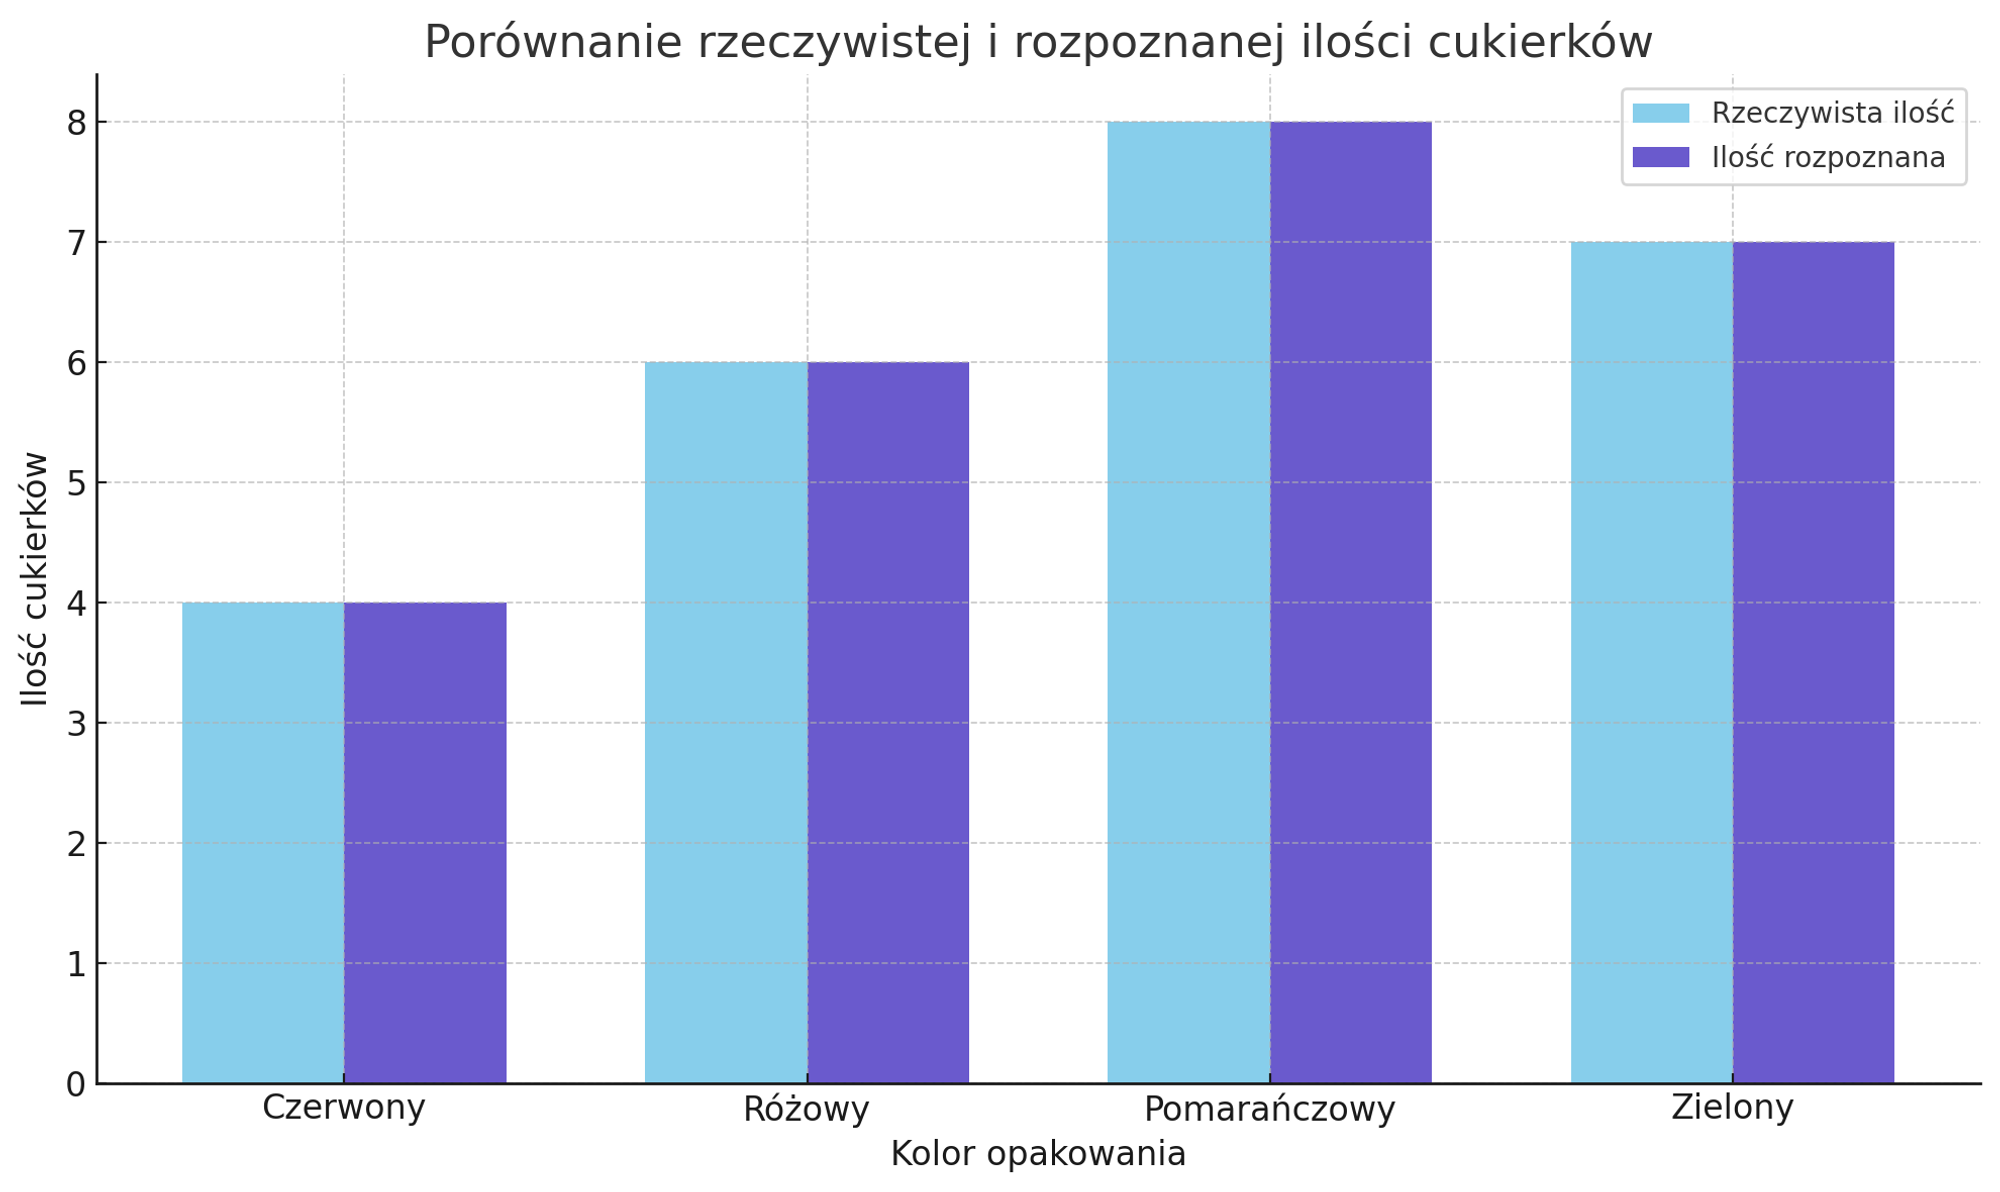
\includegraphics[width=\linewidth]{wykres1.png}
\end{center}

Jak widać, nasza metoda dla nagrania 1. (który jest zgodny z wyżej wyjaśnioną konfiguracją stanowiska pomiarowego) daje wyniki 100-tu procentowej zgodności między rzeczywistą ilością cukierków, a tą rozpoznaną przez program, dla danego koloru opakowania cukierka.

Nagranie to pokazuje poprawne działanie metody, nawet w sytuacji, gdy na linii zliczającej kolor cukierka znajdują się jednocześnie dwa cukierki, jeden pod drugim.

\begin{center}
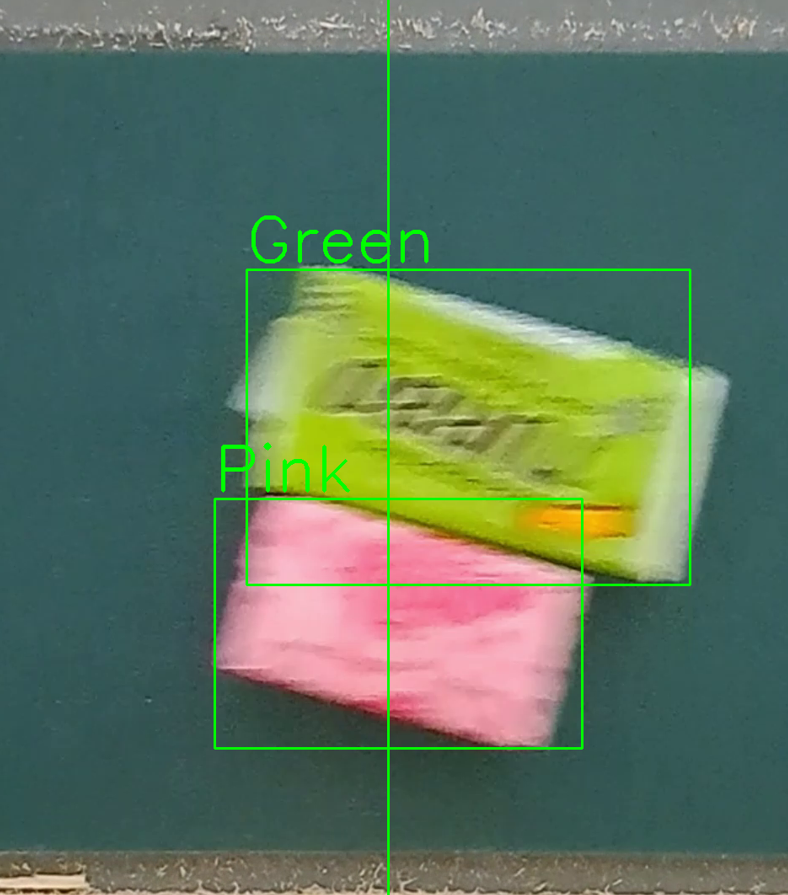
\includegraphics[width=6cm]{badanie.png}
\end{center}

\subsection{Nagranie 2}


\begin{center}
\begin{tabular}{|p{0.15\linewidth}|p{0.25\linewidth}|p{0.25\linewidth}|p{0.25\linewidth}|}
 \hline
 Kolor opakowania & Rzeczywista ilość cukierków & Ilość cukierków rozpoznana przez metodę & Procent rozpoznanych cukierków \\
 \hline
 Czerwony & 7 & 6 & 85\% \\
 \hline
 Różowy & 8 & 7 & 87\% \\
 \hline
 Pomarańczowy & 8 & 7 & 87\% \\
 \hline
 Zielony & - & - & -\% \\
 \hline
\end{tabular}
\end{center}

\begin{center}
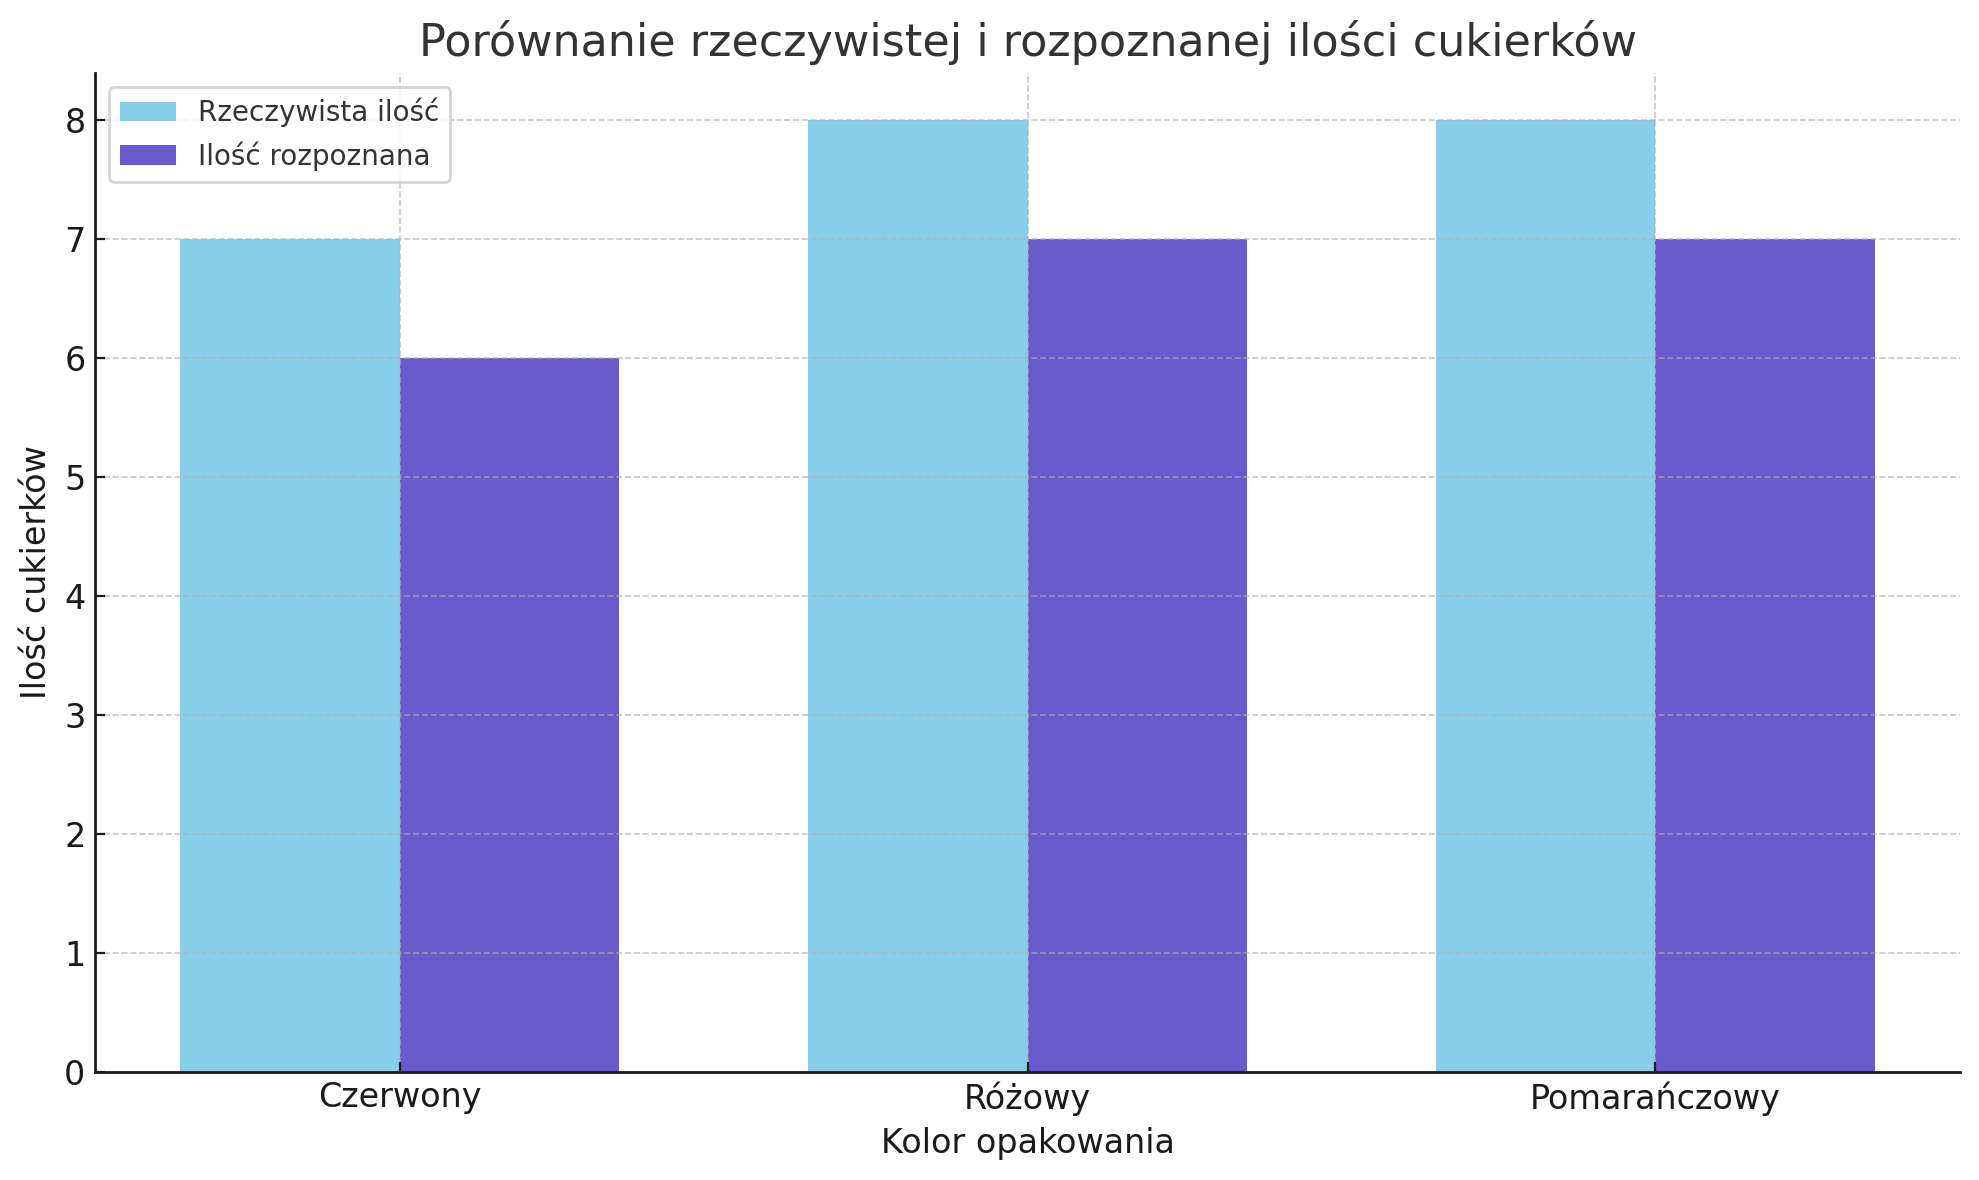
\includegraphics[width=\linewidth]{wykres2.png}
\end{center}

Nagranie 2. nie posiada żadnych cukierków z zielonym kolorem opakowania, więc zostały wyłączone z dyskusji na tym przykładzie.

Na tym nagraniu nasz program nie osiągnął 100\% w żadnym z obserwowanych kolorów. Niedokładność ta w każdym przypadku była spowodowana przez ten sam przypadek. Ponieważ nasza metoda klasyfikuje cukierek tylko na podstawie jego koloru, program ma problem z rozpoznaniem dwóch cukierków tego samego koloru znajdujących się bezpośrednio obok siebie (stykających się ze sobą). Na nagraniu 1. przypadek ten nie wystąpił, stąd otrzymaliśmy początkowo idealną dokładność.

\begin{center}
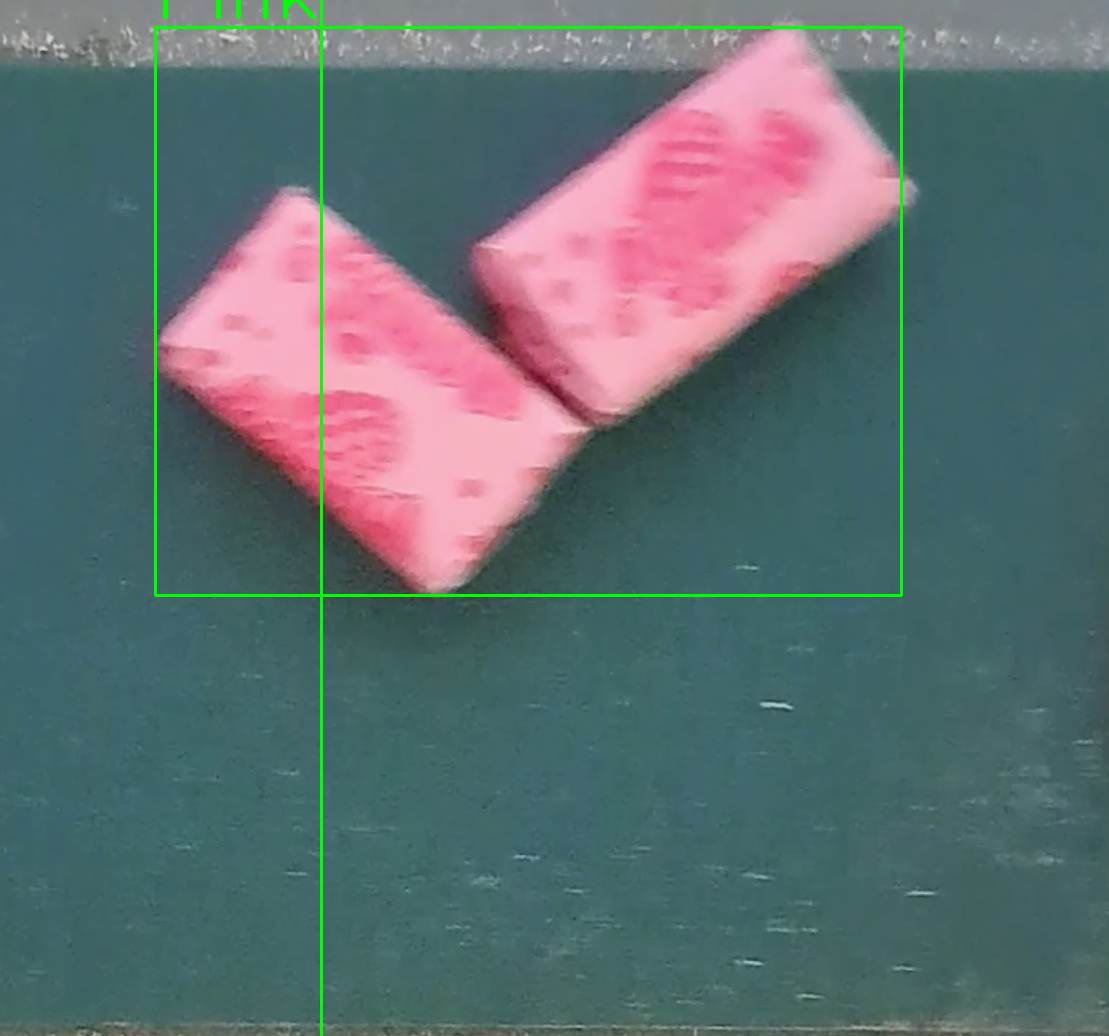
\includegraphics[width=0.3\linewidth]{pink.png}
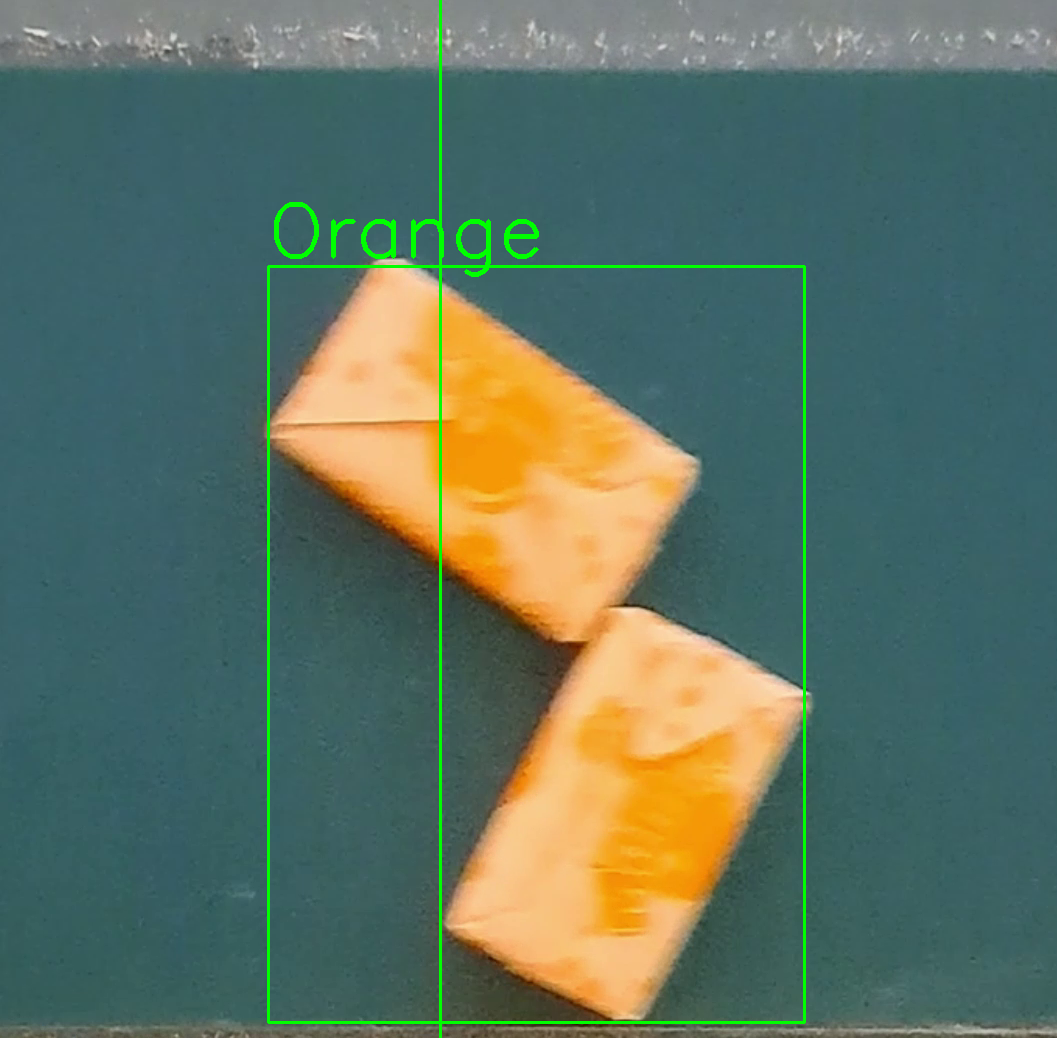
\includegraphics[width=0.3\linewidth]{orange.png}
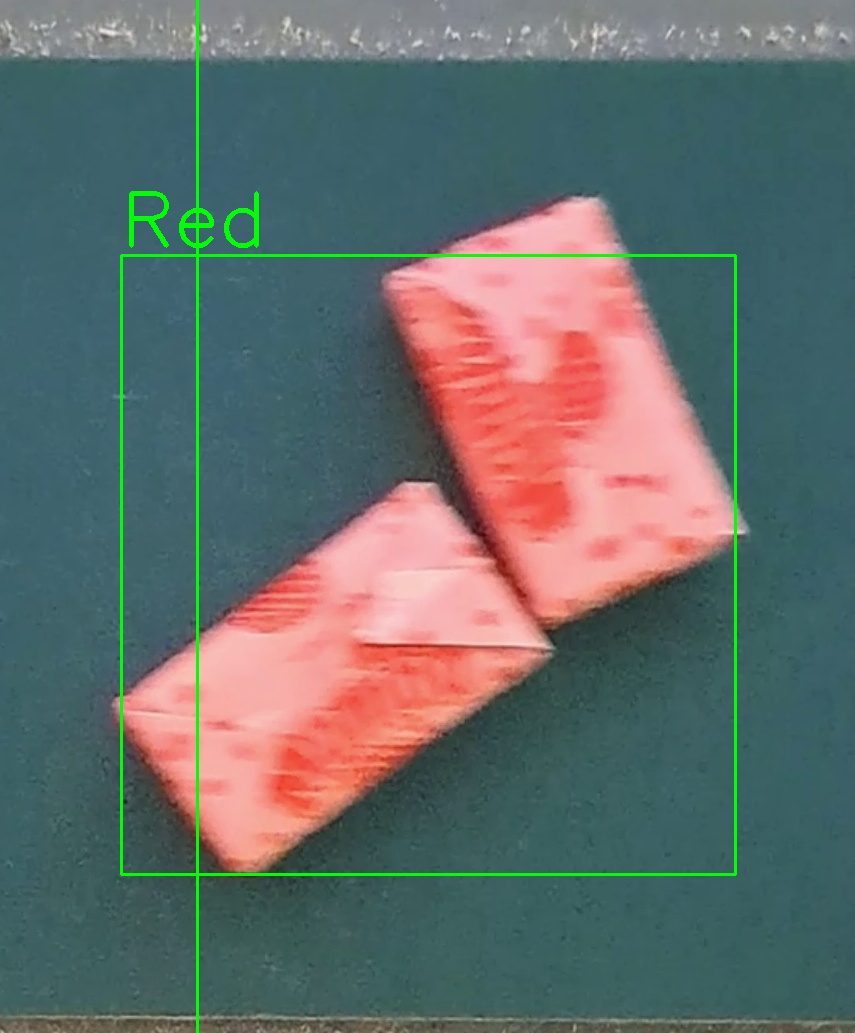
\includegraphics[width=0.3\linewidth]{red.png}
\end{center}

\subsection{Skuteczność metody na podstawie obu nagrań}

Łącznie na obu nagraniach wystąpiło 48 cukierków, z czego poprawnie rozpoznano 45 z nich. Daje nam to średnią dokładność 94\%. Aby otrzymać jak najlepsze wyniki warto zadbać o różnorodność kolorów opakowań cukierkó na taśmie znajdujących się bezpośrednio nad czytnikiem w danej chwili.

\section{Wnioski}
\label{Wnioski}

Metoda została zaprojektowana w celu zliczania ilości cukierków na podstawie koloru ich opakowań na nagraniu. Uzyskane wyniki były zgodne z założeniami projektu. Skuteczność rozpoznawania cukierków po opakowaniach wynosiła 94\%, a precyzja wahała się w granicach +/- 2 cukierki.

Analiza dokładności rozwiązania wykazała, że system skutecznie identyfikuje cukierki o różnych kolorach dla określonego rozmiaru minimalnego.

Podczas działania programu zostaje wykorzystywane około 200MB pamięci RAM. Jednakże większe zużycie zasobów wystąpiło na procesorze 30\% - 45\% mocy obliczeniowej. Nie wpłynęło to w żaden sposób na pracę komputera ani programu, nie wystąpiły spowolnienia systemu, a program działał bez żadnych spowolnień ani błędów.

Rozwiązanie to możne znaleźć zastosowanie w branży spożywczej do zliczania ilości cukierków.

\section{Literatura}
\label{Literatura}
\begin{thebibliography}{9}

\bibitem{opencv1}
\url{https://docs.opencv.org/3.4/d8/dfe/classcv_1_1VideoCapture.html#a949d90b766ba42a6a93fe23a67785951}

\bibitem{opencv2}
\url{https://docs.opencv.org/3.4/d8/dfe/classcv_1_1VideoCapture.html#a9d2ca36789e7fcfe7a7be3b328038585}

\bibitem{opencv3}
\url{https://docs.opencv.org/3.4/d8/dfe/classcv_1_1VideoCapture.html#a473055e77dd7faa4d26d686226b292c1}

\bibitem{opencv4}
\url{https://docs.opencv.org/3.4/d8/d01/group__imgproc__color__conversions.html#ga397ae87e1288a81d2363b61574eb8cab}

\bibitem{opencv5}
\url{https://docs.opencv.org/3.4/d7/dfc/group__highgui.html#ga453d42fe4cb60e5723281a89973ee563}

\bibitem{opencv6}
\url{https://docs.opencv.org/3.4/d7/dfc/group__highgui.html#ga5628525ad33f52eab17feebcfba38bd7}

\bibitem{opencv7}
\url{https://docs.opencv.org/3.4/d6/d6e/group__imgproc__draw.html#ga5126f47f883d730f633d74f07456c576}

\bibitem{opencv8}
\url{https://docs.opencv.org/3.4/d3/dc0/group__imgproc__shape.html#ga17ed9f5d79ae97bd4c7cf18403e1689a}

\bibitem{opencv9}
\url{https://docs.opencv.org/3.4/d3/dc0/group__imgproc__shape.html#ga2c759ed9f497d4a618048a2f56dc97f1}

\bibitem{opencv10}
\url{https://docs.opencv.org/3.4/d3/dc0/group__imgproc__shape.html#ga103fcbda2f540f3ef1c042d6a9b35ac7}

\bibitem{opencv11}
\url{https://docs.opencv.org/3.4/d2/de8/group__core__array.html#ga48af0ab51e36436c5d04340e036ce981}

\bibitem{opencv12}
\url{https://docs.opencv.org/3.4/d6/d6e/group__imgproc__draw.html#ga07d2f74cadcf8e305e810ce8eed13bc9}

\bibitem{opencv13}
\url{https://docs.opencv.org/3.4/d8/dfe/classcv_1_1VideoCapture.html#afb4ab689e553ba2c8f0fec41b9344ae6}

\bibitem{opencv14}
\url{https://docs.opencv.org/3.4/d7/dfc/group__highgui.html#ga6b7fc1c1a8960438156912027b38f481}

\bibitem{opencv15}
\url{https://docs.opencv.org/3.4/d7/d1b/group__imgproc__misc.html#gae8a4a146d1ca78c626a53577199e9c57}

\bibitem{opencv16}
\url{https://docs.opencv.org/3.4/d6/d6e/group__imgproc__draw.html#ga7078a9fae8c7e7d13d24dac2520ae4a2}

\bibitem{virtuslab}
\url{https://virtuslab.com/case-study/object-detection-in-real-time-streaming-recordings-and-images}

\bibitem{gfg}
\url{https://www.geeksforgeeks.org/detect-an-object-with-opencv-python/}

\bibitem{dry}
\url{https://dontrepeatyourself.org/post/color-based-object-detection-with-opencv-and-python/}

\bibitem{yt-motorcycle}
\url{https://www.youtube.com/watch?v=O3b8lVF93jU/}

\bibitem{yt-banana}
\url{https://www.youtube.com/watch?v=aFNDh5k3SjU&t=1004s/}

\bibitem{chocolates}
\url{https://blog.roboflow.com/identifying-chocolates-with-computer-vision/}

\bibitem{vending}
 \url{https://www.researchgate.net/publication/337068624_Towards_Identification_of_Packaged_Products_via_Computer_Vision_Convolutional_Neural_Networks_for_Object_Detection_and_Image_Classification_in_Retail_Environments}

\end{thebibliography}

\end{document}